\section{Proofs}\label{app:proofs}

\begin{proposition}
  The language of compressed terms is strongly normalizing.
\end{proposition}

\begin{proof}
  Consider evaluating $\hat{t}$ in applicative order (leftmost innermost).
  %
  In this case, any left-hand size of a $\beta$-reduction has no inner $\beta$-redexes.
  %
  Since in our language a $\lambda$-abstraction can only be on the left-hand side of a $\beta$-redex,
  it means that expression being reduced has no inner $\lambda$-abstractions.
  %
  For that reason, the number of $\lambda$-abstractions in an expression strictly decreases with every $\beta$-step
  (the sole one in the reduced redex disappears, and all other $\lambda$-abstractions are outside of the reduced redex, and hence unchanged).
\end{proof}

\begin{lemma}
Given a $\kappa$-step $\hat{t}_1 \rwsteps{\kappa(p')} \hat{t}_2$
  if a pattern $p$ has $N$ matches in $\hat{t}_2$, it also has at least $N$ matches in $\hat{t}_1$.
  \label{lem:pat-match}
\end{lemma}
\begin{proof}
  There are four cases for what $p$ can match in $\hat{t}_2$:
  \begin{itemize}
  \item a subterm that does not overlap with the newly introduced $\beta$-redex: in this case, the match is unaffected by the $\kappa$-step;
  \item a subterm inside an actual argument of the $\beta$-redex: this actual argument becomes a sub-term of $\hat{t}_1$;
  \item a sub-term inside the body of the $\beta$-redex: $\hat{t}_1$ has a sub-term that is more specific than the body, and hence still matches $p$;
  \item a sub-term that includes the entire $\beta$-redex inside: since $p$ is first order, it cannot mention the redex, so the redex must be contained entirely inside the substitution; 
  hence again the match is unaffected by the $\kappa$-step.
  \end{itemize}
\end{proof}

\begin{theorem}[Soundness and Completeness of Pattern-Based Library Learning]
  For any term $t \in \termsof{\Sigma}$ and compressed term $\hat{t} \in \absof{\Sigma}{\mathcal{X}}$:
  \begin{description}[font=\itshape]
    \item[(Soundness)] If $t$ compresses into $\hat{t}$, then $\hat{t}$ evaluates to $t$: $\forall \patset . t \rewrites{\kappa(\patset)} \hat{t} \Longrightarrow \hat{t} \evals t$.
    \item[(Completeness)] If $\hat{t}$ is a solution to the (global) library learning problem, 
    then $t$ compresses into $\hat{t}$ using only patterns that have a match in $t$:
    $\hat{t} \in \argmin_{\hat{t}' \evals t} \sz(\hat{t}') \Longrightarrow t \rewrites{\kappa(\patset)} \hat{t}$, 
    where $\patset = \{p \in \patsof{\Sigma}{\mathcal{X}} \mid t' \in \subterms(t) , t' \sub p\}$.
  \end{description}
\label{thm:pat-lib-learning-app}
\end{theorem} 

\begin{proof}
The soundness is trivial because inverting any $\kappa$-rewrite gives a valid $\beta$-reduction.

The other direction (completeness) is more involved.
%
First let us prove that $\hat{t}$ can be obtain by any compression, regardless of whether the patterns occur in $t$.
%
This is non-trivial
because inverting a $\beta$-reduction $(\lambda \many{X} \bnd \hat{t}_1)\ \many{\hat{t}_2}  \betared  \hat{t}'$
does not always correspond to a well-form $\kappa$-step,
for two reasons:
(a) $\hat{t}_1$ itself contains $\lambda$-abstractions (and hence does not correspond to a pattern);
(b) $\many{X} \neq \fv(\hat{t}_1)$.
%
To overcome point (a), note that in an applicative evaluation,
both $\hat{t}_1$ and $\hat{t}_2$ contain no $\beta$-redexes (and hence no $\lambda$-abstractions).
%
Hence  $\hat{t}_1$ is a valid pattern.

For point (b), there are two cases: either (1) $\fv(\hat{t}_1) \subsetneq \many{X}$
or (2) $\fv(\hat{t}_1) \supsetneq \many{X}$.
%
Consider case (1).
%
In this case, the compressed term $\hat{t}$ has $\lambda$-bindings that are not used in their bodies.
%
Such a term cannot possibly be minimal.
% because adding unused bindings does not change the body of the lambda, 
% it cannot create more sharing, only less.
%
Removing unused bindings makes each individual $\beta$-redex smaller and cannot remove sharing,
so it always makes the overall term smaller as well.

Now consider case (2).
%
This means that $\lambda \many{X} \bnd \hat{t}_1$ has free variables, 
which must be defined in outer $\lambda$-abstractions.
%
However, using such a $\lambda$-abstraction contradicts the assumption that we are only interested in global library learning.

Finally, let us prove that all patterns used in the compression have a match in $t$.
%
Consider a compression $t = \hat{t}_0 \rwsteps{\kappa(p_1)} \hat{t}_1 \dots \rwsteps{\kappa(p_n)}  \hat{t}_n = \hat{t}$.
%
Clearly, each pattern $p_i$ has a match in the (compressed) term $\hat{t}_{i-1}$, by definition of the $\kappa$-rewrite.
%
Hence, it also occurs in $t$, by induction using Lemma~\ref{lem:pat-match}.
\end{proof}



\newpage
\section{Additional Experiments}\label{app:eval}

\begin{figure}[h]
  \centering
  \begin{subfigure}{0.48\linewidth}
    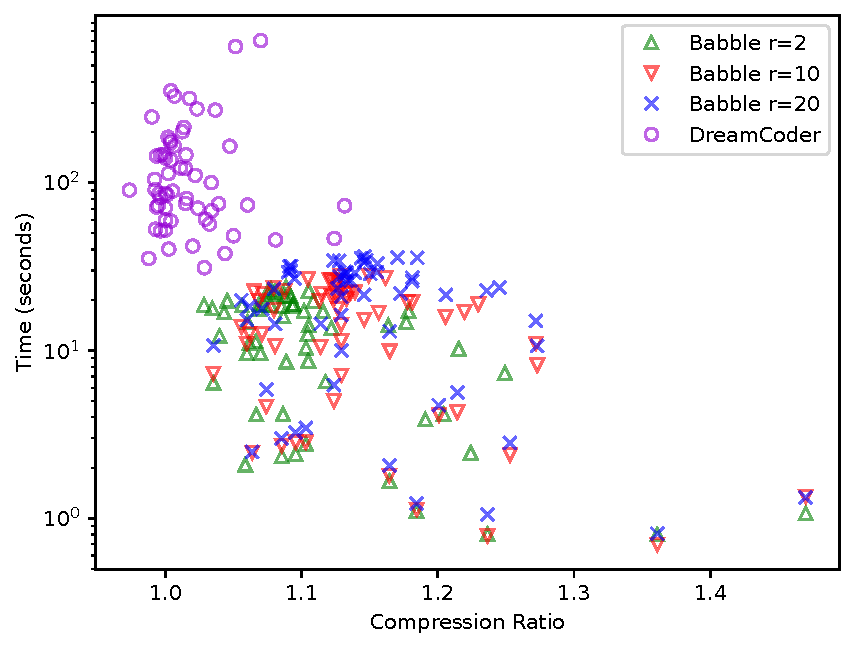
\includegraphics[width=\linewidth]{figures/scatter/list-rounds.pdf}
    \caption{List domain}
  \end{subfigure}
  \hfill
  \begin{subfigure}{0.48\linewidth}
    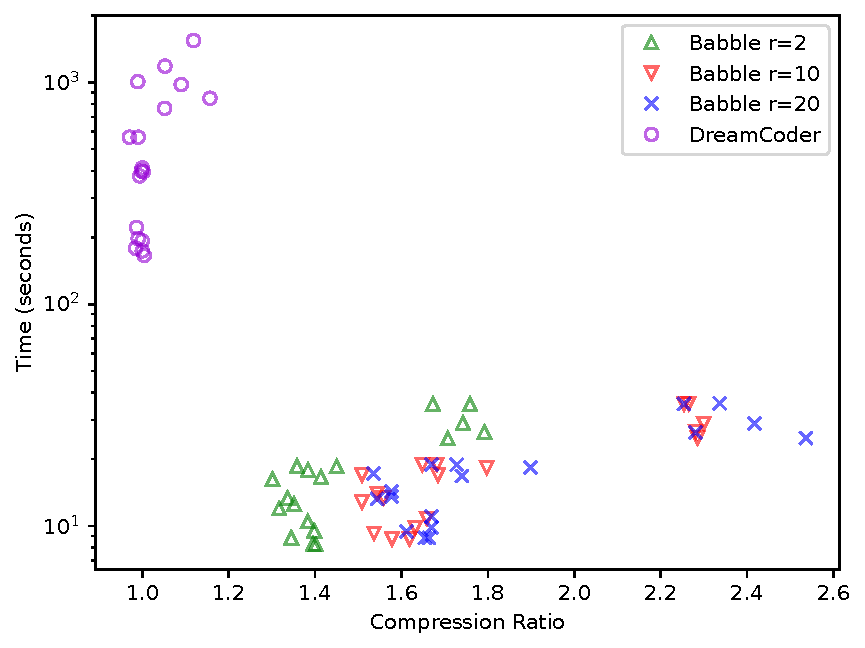
\includegraphics[width=\linewidth]{figures/scatter/physics-rounds.pdf}
    \caption{Physics domain}
  \end{subfigure}

  \begin{subfigure}{0.48\linewidth}
    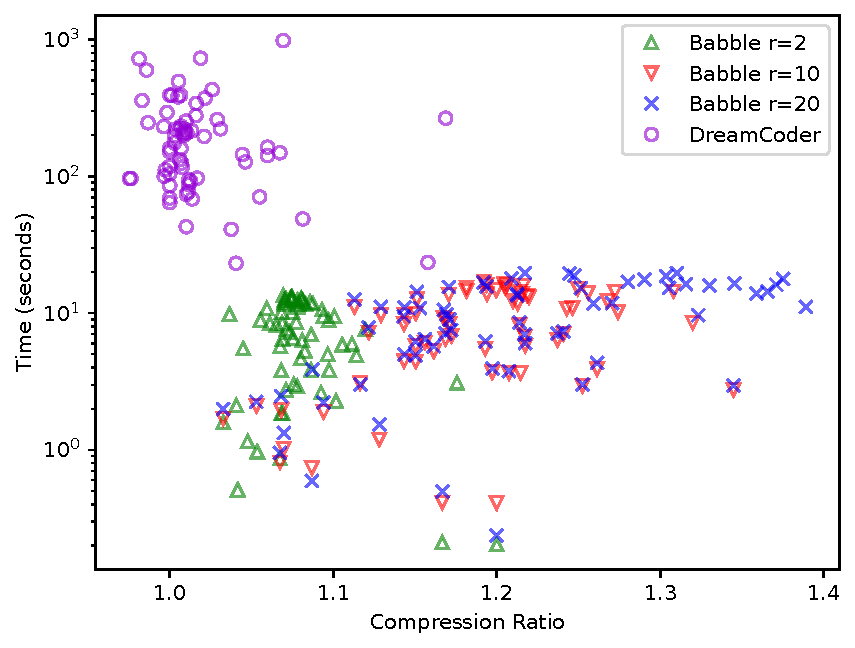
\includegraphics[width=\linewidth]{figures/scatter/text-rounds.pdf}
    \caption{Text domain}
  \end{subfigure}
  \hfill
  \begin{subfigure}{0.48\linewidth}
    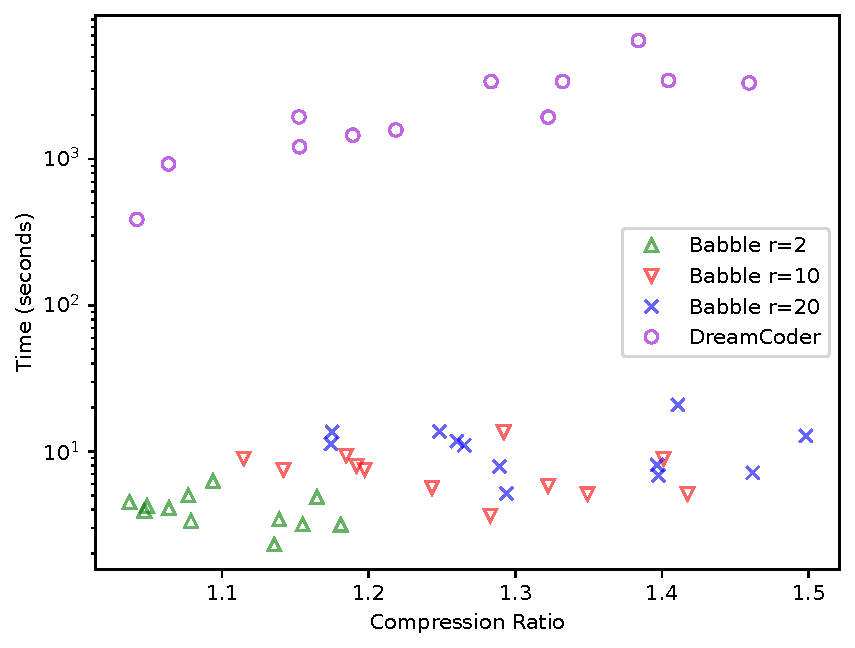
\includegraphics[width=\linewidth]{figures/scatter/logo-rounds.pdf}
    \caption{Logo domain}
  \end{subfigure}

  \begin{subfigure}{0.48\linewidth}
    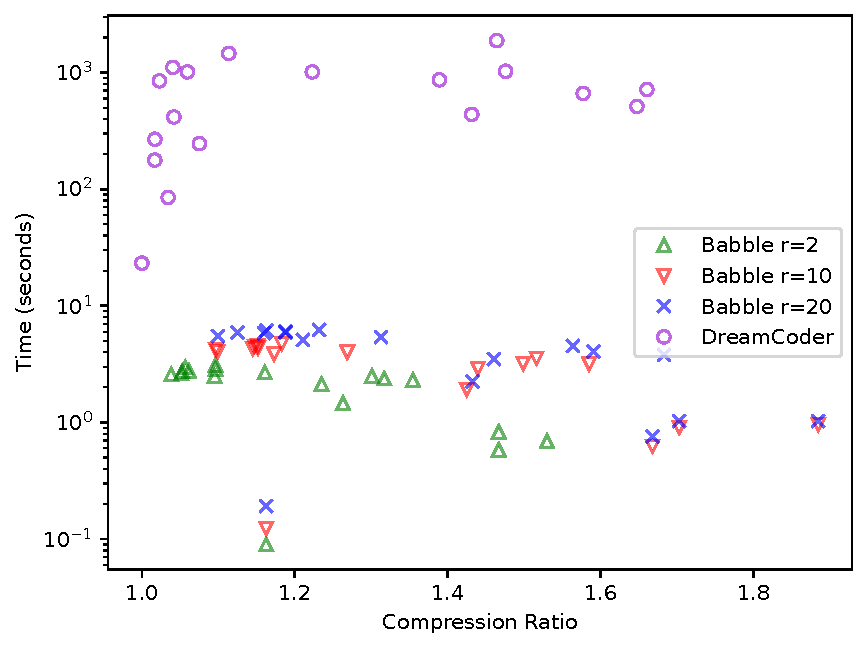
\includegraphics[width=\linewidth]{figures/scatter/towers-rounds.pdf}
    \caption{Towers domain}
  \end{subfigure}
  \caption{
    \tool's default configuration runs for 20 rounds (r=20)
    to learn additional library functions.
    This plot shows the data from \autoref{fig:dc-domains},
     but with additional \tool configuration running fewer rounds.
    With fewer rounds, \tool runs faster but compresses worse.
  }\label{fig:dc-domains-rounds}
\end{figure}